\chapter{Experimental Results of abnormalities findings and landmark detection for endoscopic images}
\label{chap-experiment-endoscopy} 
\begin{ChapAbstract}
In this chapter, we describe the dataset, task descriptions as well as the evaluation metrics used in both following challenges: The 2018 Multimedia for Medicine Task and and The Biomedia ACM MM Grand Challenge 2019. We not only report our official results provided by organizers but also discuss about the performance of each component in our algorithm by trying different experiment configurations and analyze the corresponding results.
\end{ChapAbstract}

\section{Dataset and evaluation metrics}
\label{dataset_evaluation_endoscopy}
\subsection{Dataset}
\subsubsection*{Dataset description}
According to organizers of The 2018 Multimedia for Medicine Task, the offical dataset contains a multi-class set of frames and videos for at least 4 different diseases, at least 4 different landmarks and at least 2 different findings. Each class will consist of at least 1000 frames and at least 2 short videos. The training set will be released with ground truth. All the frames in training set will be labelled with corresponding class-label. Up to 10\% of training set frames will have a detailed ground truth masks showing the exact location of disease or finding within the frame. The ground truth is collected with the help of GI endoscopists from our partner hospitals. The pre-extracted visual features such as global image features, namely: JCD, Tamura, ColorLayout, EdgeHistogram, AutoColorCorrelogram and PHOG are also included in this dataset.

\subsubsection*{Classes}
Totally, there are 16 classes of abnormal symptoms and landmark of human's gastrointestinal track (GI track). The visualisation of landmark's corresponding position in the GI track are shown in Figure \ref{fig:vis_16_classes}. As given  in the figure, the \textit{esophagitis, normal z-line, normal  pylorus, ulcerative colitis, colon, normal cecum, retroflex-stomach, retroflex-rectum and stool (plenty/inclusion)} are classes which illustrate the landmark in human's GI Track. Noticeably, the \textit{esophagitis} and \textit{normal z-line} share a same anatomical position. However, the class \textit{esophagitis} (marked with a red bounding box) refers to an  abnormal situation and \textit{normal z-line} (marked with a green bounding box) appears in normal people's GI track. Similarly, the \textit{ulcerative colitis} (marked with a red bounding and \textit{colon} (marked with a green bounding box)  refer to an abnormal and a normal situation respectively.

Besides, the \textit{dyed-lifted-polyps, dyed-resection-margins, polyps} and \textit{instruments} are abnormal symptoms that can be appeared at any position in the human's GI track. In addition, the \textit{polyp} is a  living entity in the GI track, doctors can inject some chemical component in order to demolish polyps. This chemical changes polyp's color to white, which became the \textit{dyed-lifted polyps}. After that, doctors will use some special \textit{instruments} to remove the polyp completely, the remains are \textit{dyed-resection-margins}. 

\begin{figure}[thb]
\begin{center}
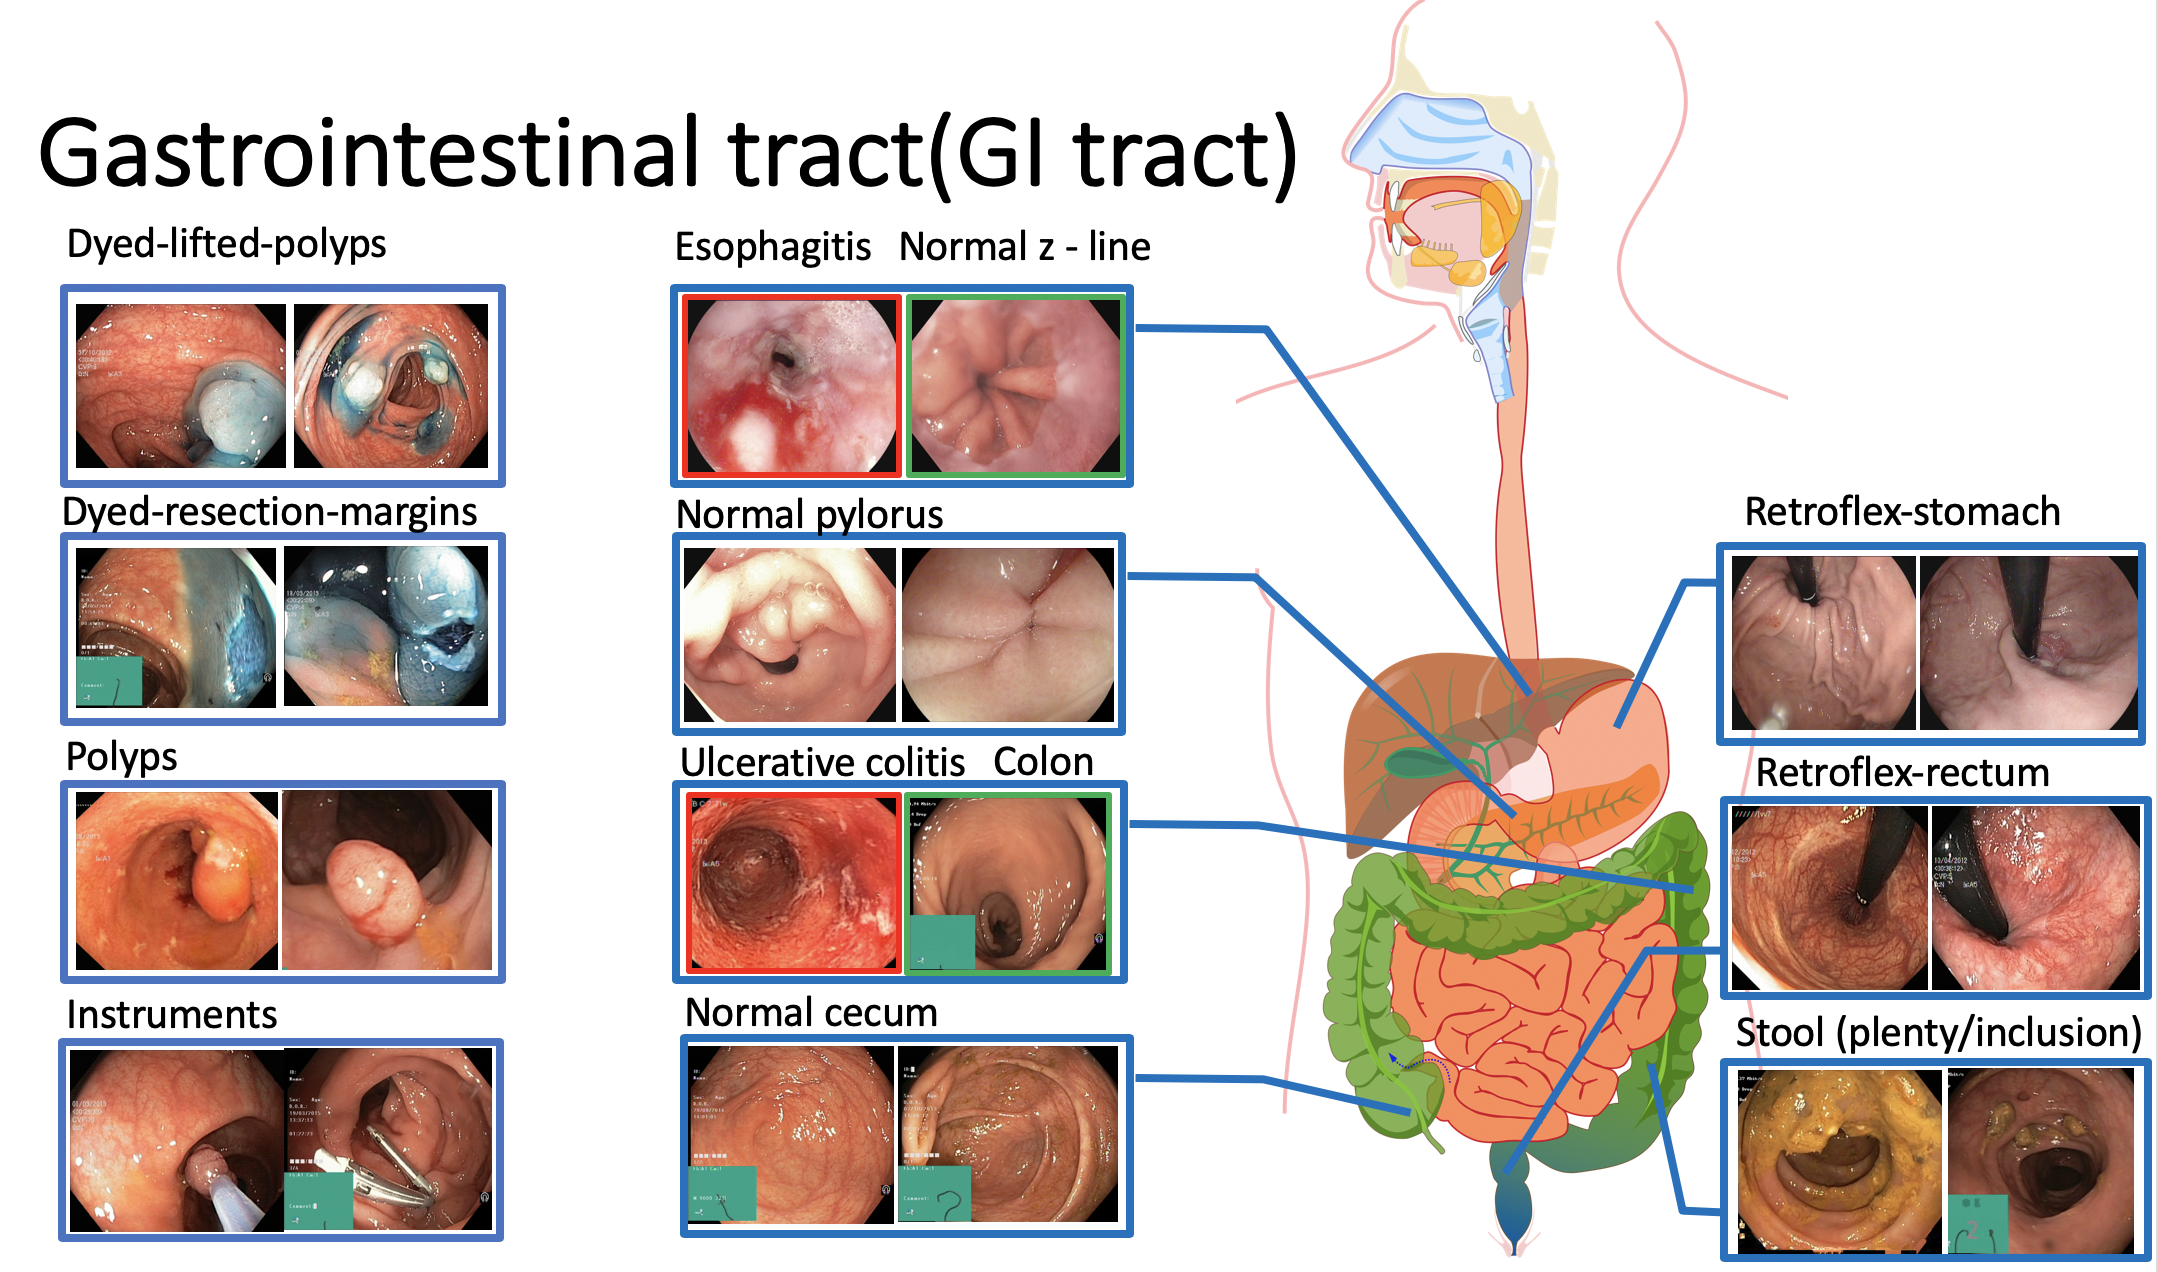
\includegraphics[width=\textwidth]{endoscopy_resources/vis_16_classes.png}
\end{center}
   \caption{Classes of the Medico: The 2018 Multimedia for Medicine Task official dataset and their corresponding order in the Gastrointestinal track.}
\label{fig:vis_16_classes}
\end{figure}

\subsubsection*{Multi-classes classification}
When we conducting our experiments on this dataset, we find out that both the development set and the test test contain a number of images can be classified into several classes simultaneously. After noticing the task organizers for this problem, they define a priority list according to the important level of that finding during the endoscopy screening process. The list is given bellow in descending important level (most important to less important):

\begin{multicols}{3}
\begin{enumerate}
    \item out-of-patient
    \item instruments
    \item dyed-lifted-polyps
    \item dyed-resection-margins
    \item polyps
    \item esophagitis
    \item ulcerative-colitis
    \item retroflex-rectum
    \item retroflex-stomach
    \item normal-cecum
    \item normal-pylorus
    \item normal-z-line
    \item stool-plenty
    \item stool-inclusions
    \item colon-clear
    \item blurry-nothing
\end{enumerate}
\end{multicols}

\subsubsection*{Development Set and Test Set}
In this challenge, task organizers divide this 16-classes dataset into two sub-set: \textit{the development set} consists of 5293 images  and the  \textit{test set} consits of 8740 images. Only the image's label of the \textit{development set} are visible to participants.

\subsection{Evaluation metrics}
Regarding to the evaluation process, task organizers propose several metrics for each sub-task. Totally, there are four sub-tasks can be conducted on this dataset, including \textit{Classification of diseases and findings}, \textit{fast and efficient classification}, \textit{basic reporting} and \textit{advance reporting}. In our work, we evaluate our approaches on the first and the second sub-task. The remain sub-tasks are not conducted by our team or others and they are left for future development.
\begin{itemize}
    \item \textbf{Classification of diseases and findings:} The evaluation metric is the multiclass version of the Mathews Correlation Coefficient (MCC) \cite{MATTHEWS1975442}, which captures the quality of classification as reflected in the correlation between the ground truth and the classifier's predictions. The MCC can be calculated directly from the confusion matrix using the formula:
    \begin{equation}
        MCC = \frac{TP \times TN - FP \times FN }{\sqrt{(TP + FP)(TP + FN)(TN + FP)(TN + FN)}}
    \end{equation}
        
    where $TP$ stands for the number of true positives, $TN$ is the number of true negatives, $FN$ is the number of false negatives and $FP$ is the number of true negatives.
    \item \textbf{Fast and efficient classification:} Participants of this sub-task are asked to run the code on a standard PC and provide information about hardware used. The time from input to output will be measured and weighed by the accuracy of the output. Participants are also asked to record the amount of training data used. The amount of training data will also be weighted by the accuracy of the output.
    \item \textbf{Reporting (exploratory/optional):} The metric will reflect the completeness and the correctness of the summary. This sub-task allows organizers to focus on understanding the performance of the automatic systems in practice (from the point of view of the medical expert). However, this sub-task is currently an optional sub-task.

    \item \textbf{Advanced reporting (exploratory/optional):} In order to evaluate participant's result on this sub-task, two medical partners will participate in the evaluation process in terms of how useful it is for them and if it satisfies existing demands for documentation of endoscopic procedures. Similar to  the above sub-task, this sub-task is also an optional sub-task.
\end{itemize}

\section{Experimental setup} 
\label{sec:endscopy_setup}
\subsection{Re-labeling Medico Development Dataset}
After training with the development set of Medico 2018 challenge, we find some issues related to some training samples in the given dataset. Firstly, with a help of a medical student, we found out that there are inappropriate labels according between different classes. Secondly, there are several samples in the development set that conflict with the priority list that the organizers proposed. Therefore, in order to help our model to learn with the least confusing, we apply the new labels and make them as the modified version of the original dataset. We also make that modified version of the given dataset available to be contributed for the task organizers in future challenges. 

\subsection{Abnormalities localization with Faster R-CNN}
We inherited the work from Chen et al. \cite{chen17implementation} which is a Tensorflow implementation of faster RCNN detection framework. Due to the small size of abnormalities in endoscopic image dataset, we use several anchors size at $4,8,16,32$ and corresponding aspect ratios at $0.5,1,2$. ResNet 101 pre-trained model \footnote{\url{github.com/tensorflow/models/tree/master/research/slimơ\#pre-trained-models}} is used as Faster R-CNN backbone. The concepts we used to train including \textit{instruments, polyps, dyed-lifted-polyps} and \textit{dyed-resection-margins}. Original and our augmented dataset are trained simultaneously for 70000 iterations. It usually takes 5-6 hours training on GeForce GTX 1080 GPU.

In test-time inference, each image is fed through the module and we only keep bounding boxes that have confident score over $0.95$.

\subsection{ResNet Classifier and Multi-tasks Classifier}
Classifiers used in our work are implemented with PyTorch - a Python machine learning library. Original and our augmented dataset are trained simultaneously for 200 epochs with Adam optimizer \cite{DBLP:journals/corr/KingmaB14}. The learning rate is set at $10^{-3}$ and decay by a factor of $0.1$ every $10$ epochs. When training the model, we freeze every layer except the last convolution and fully connected layer. In training phase, each image is resized into a batch of 64 images with size $224\times224$ are fed into the network at each step. We also apply random horizontal flip and random crop augmentation during this phase. 
\section{Experimental results}
\subsection{Abnormalities localization with Faster R-CNN results}
According to our experiments, applying object detection model such as Faster R-CNN shows significant improvements in two situation:
\begin{itemize}
    \item In the first situation, abnormal symptoms appeared in small regions of an image, that can be easily mis-classified by the image classification module. This situation usually happens with the \textit{instruments} class. Three examples are given in Figure \ref{fig:res_frcnn_instr} where \textit{instruments} appeared in really small region at the corner of an image.
    \item In the second situation, multiple abnormal symptoms seem to appeared together in the same image. Figure \ref{fig:res_frcnn_dyed} illustrated this situation where \textit{dyed-lifted-polyps} and \textit{dyed-resection-margins} symptoms appeared together. By having information about every symptom and their position inside an image, it is easier for the system to fit with the priority list of this challenge. Besides, it also an useful source of information for future endoscopy diagnosis system that can localize the position of abnormal symptoms for doctors.  
\end{itemize} 

\begin{figure}[thb]
\begin{center}
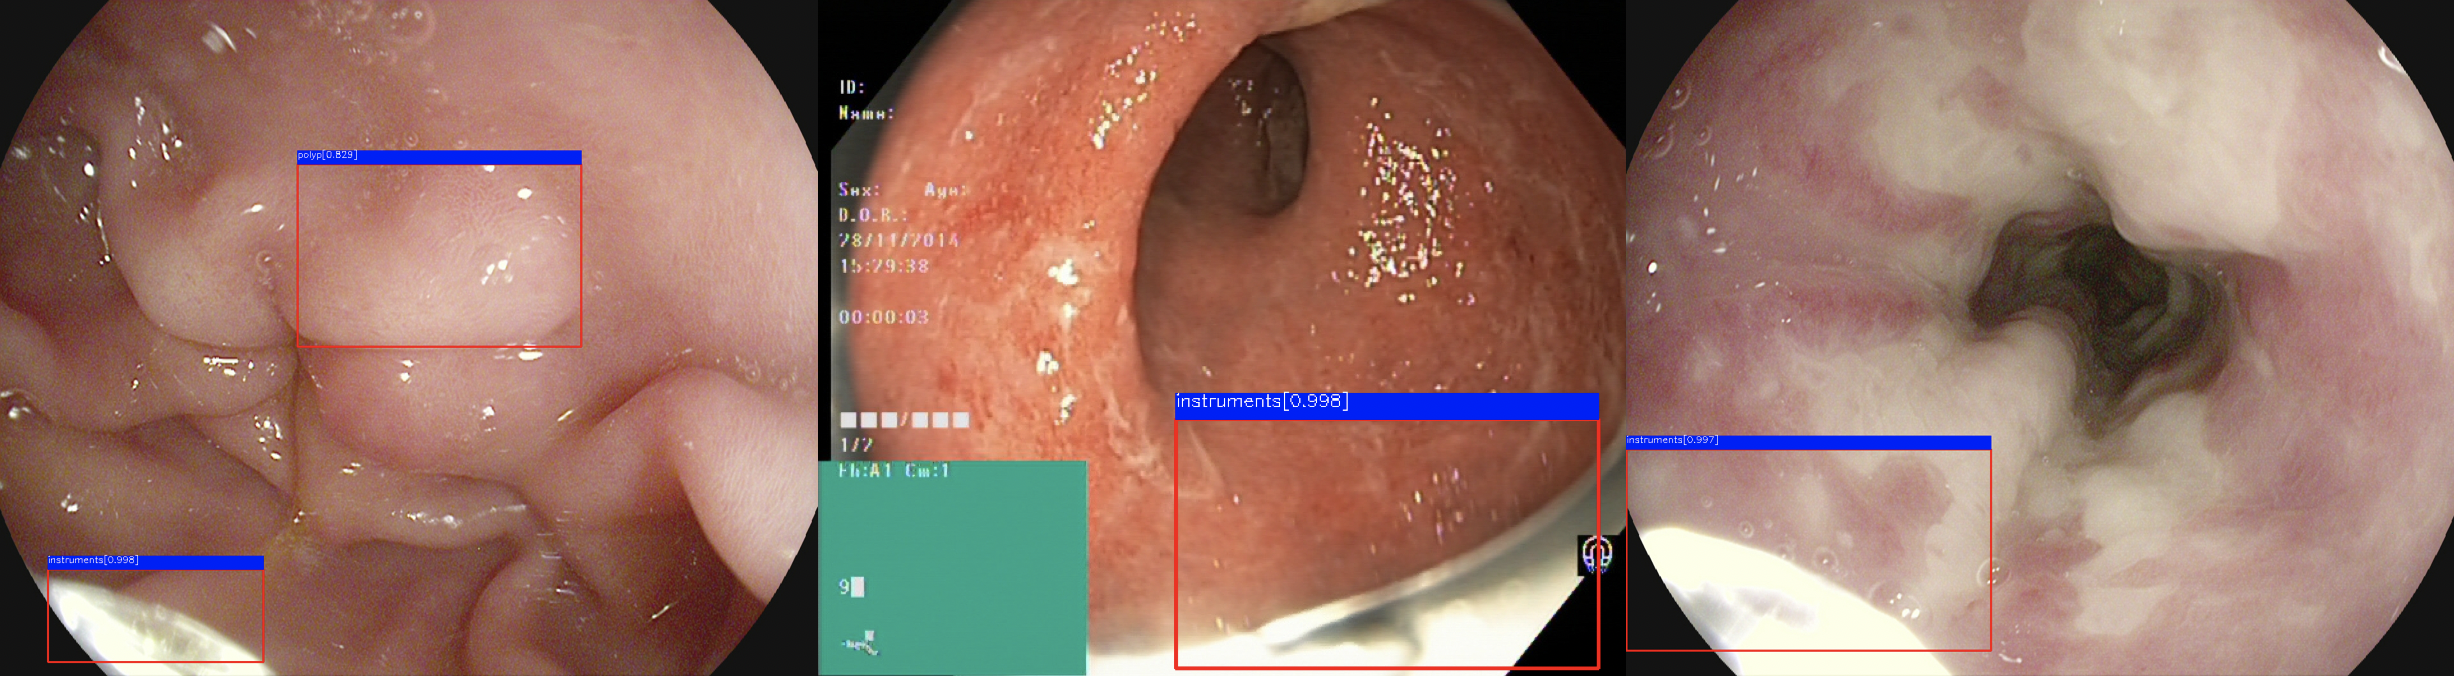
\includegraphics[width=\textwidth]{endoscopy_resources/res_frcnn_instr.png}
\end{center}
   \caption{\textit{Instrument} objects detected in endoscopic images. They are used to be mis-detected by image classification model which usually focus on global visual features.}
\label{fig:res_frcnn_instr}
\end{figure}

\begin{figure}[thb]
\begin{center}
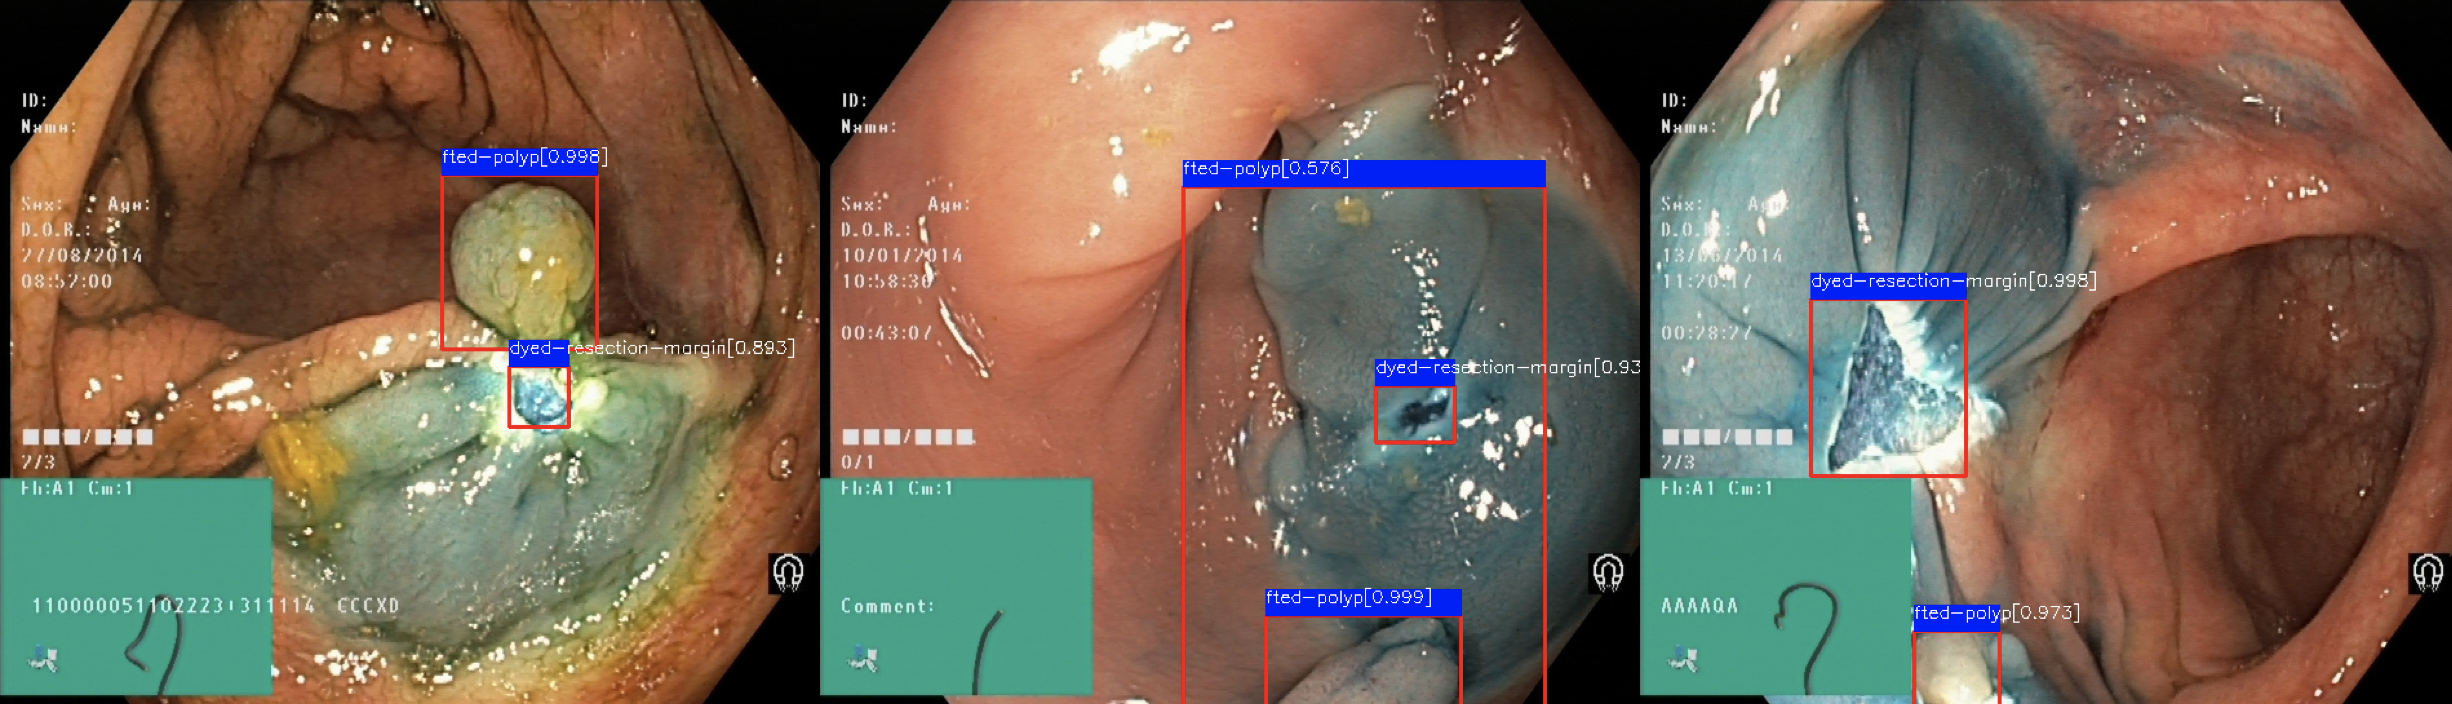
\includegraphics[width=\textwidth]{endoscopy_resources/res_frcnn_dyed_lifted_polyps.png}
\end{center}
   \caption{\textit{Dyed-lifted-polyps} and \textit{dyed-lifted-margins} symptoms detection.}
\label{fig:res_frcnn_dyed}
\end{figure}

\subsection{Medico: The 2018 Multimedia for Medicine Task - Official results}
\label{sec:medico2018_results}
Two out of three our improvements are used in the Medico: The 2018 Multimedia for Medicine Task challenge including applying object detection model on abnormal findings and dataset augmentation. Table \ref{teams_result} shows the official results of the international challenge. We received the first place winner among 10 teams around the world with the MCC score at 94.24\% and 99.33\% in term of the accuracy.

There is a trade-off between speed and accuracy when comparing the result of \textit{Run01} and \textit{Run02}. In \textit{Run02}, we reduce a large number of images passing through Faster R-CNN for the sake of time, so its performance seems to be relatively worse than \textit{Run01}'s.

As we mentioned earlier, data pre-processing takes an important role in building a deep-neural network model. Through our experiments, in the case of less training data, the augmented dataset helps us improve the performance of deep-neural network model. \textit{Run03} and \textit{Run05} show impressive results comparing to the first two runs. This implies that training on our re-labeled development set provides better models.

On the other hand, using the Residual neural network cannot classify efficiently the two classes \textit{esophagitis} and \textit{normal-z-line}. The same problem also occurs between the \textit{dyed-resection-margins} and \textit{dyed-lifted-polyps} classes. It can be observed in the confusion matrices of the two pairs (Figure \ref{fig:cfs_mat}). Therefore, these are the two main reasons which mainly bring negative impact to our results. In Figure \ref{fig:confusing}, selected samples from \textit{esophagitis} and \textit{normal-z-line} are given in order to illustrate the fine-grain situation of these classes that is challenging even for human without special knowledge to distinguish them correctly.

\begin{figure}[thb]
\begin{center}
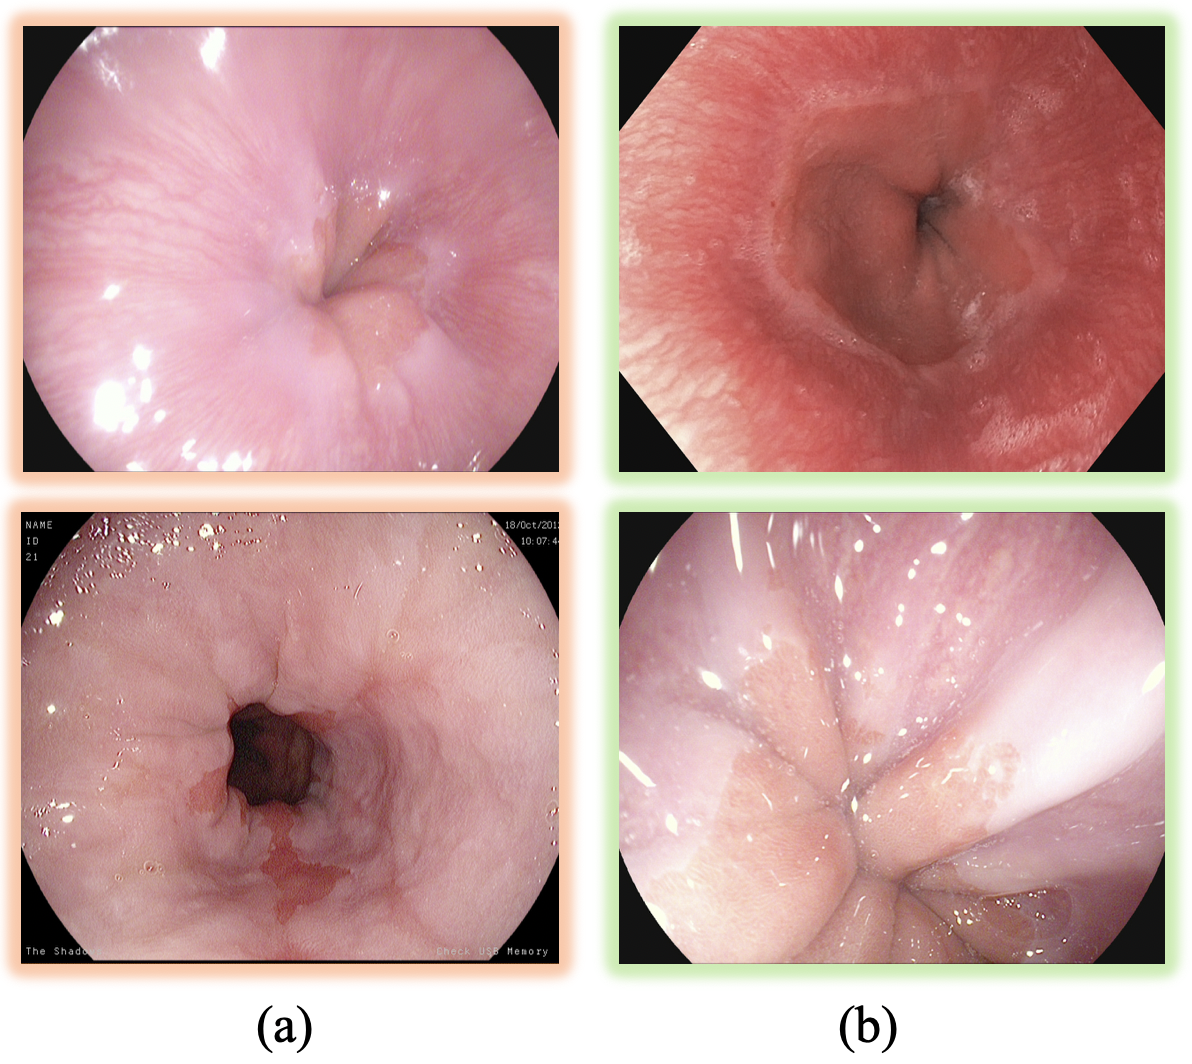
\includegraphics[width=0.8\textwidth]{endoscopy_resources/confusing_cases.png}
\end{center}
   \caption{Example of confusing cases taken from the Development Set (ground-truth provided). \textit{esophagitis} samples are marked with red box and \textit{normal-z-line} samples with green box. Two samples from the first row are harder to be distinguished than those in the second row}
\label{fig:confusing}
\end{figure}

Additionally, as we mentioned in section 3, the configuration of Run05 intuitively prefers \textit{esophagitis} to \textit{normal-z-line}, which may leads to an increasing of the false-positive cases in the result.

By comparison to the others, \textit{Run04} has the lowest precision since it uses 75\% of training data. Decreasing the amount of training samples of course affects the performance in deep-learning models. Nevertheless, the result is still acceptable when it decreases only a few percentages and its configuration is as same as \textit{Run03}. This is an evidence that we are even able to reduce up to 50\% of data when the less training time is preferred over the accuracy.

Last but not least, we performed training and testing our model on a Tesla K80 GPU. The average inference time for all images in the test set we measured for Run01 is around 150ms per image and around 43ms for others. 

\begin{figure}[thb]
\begin{center}
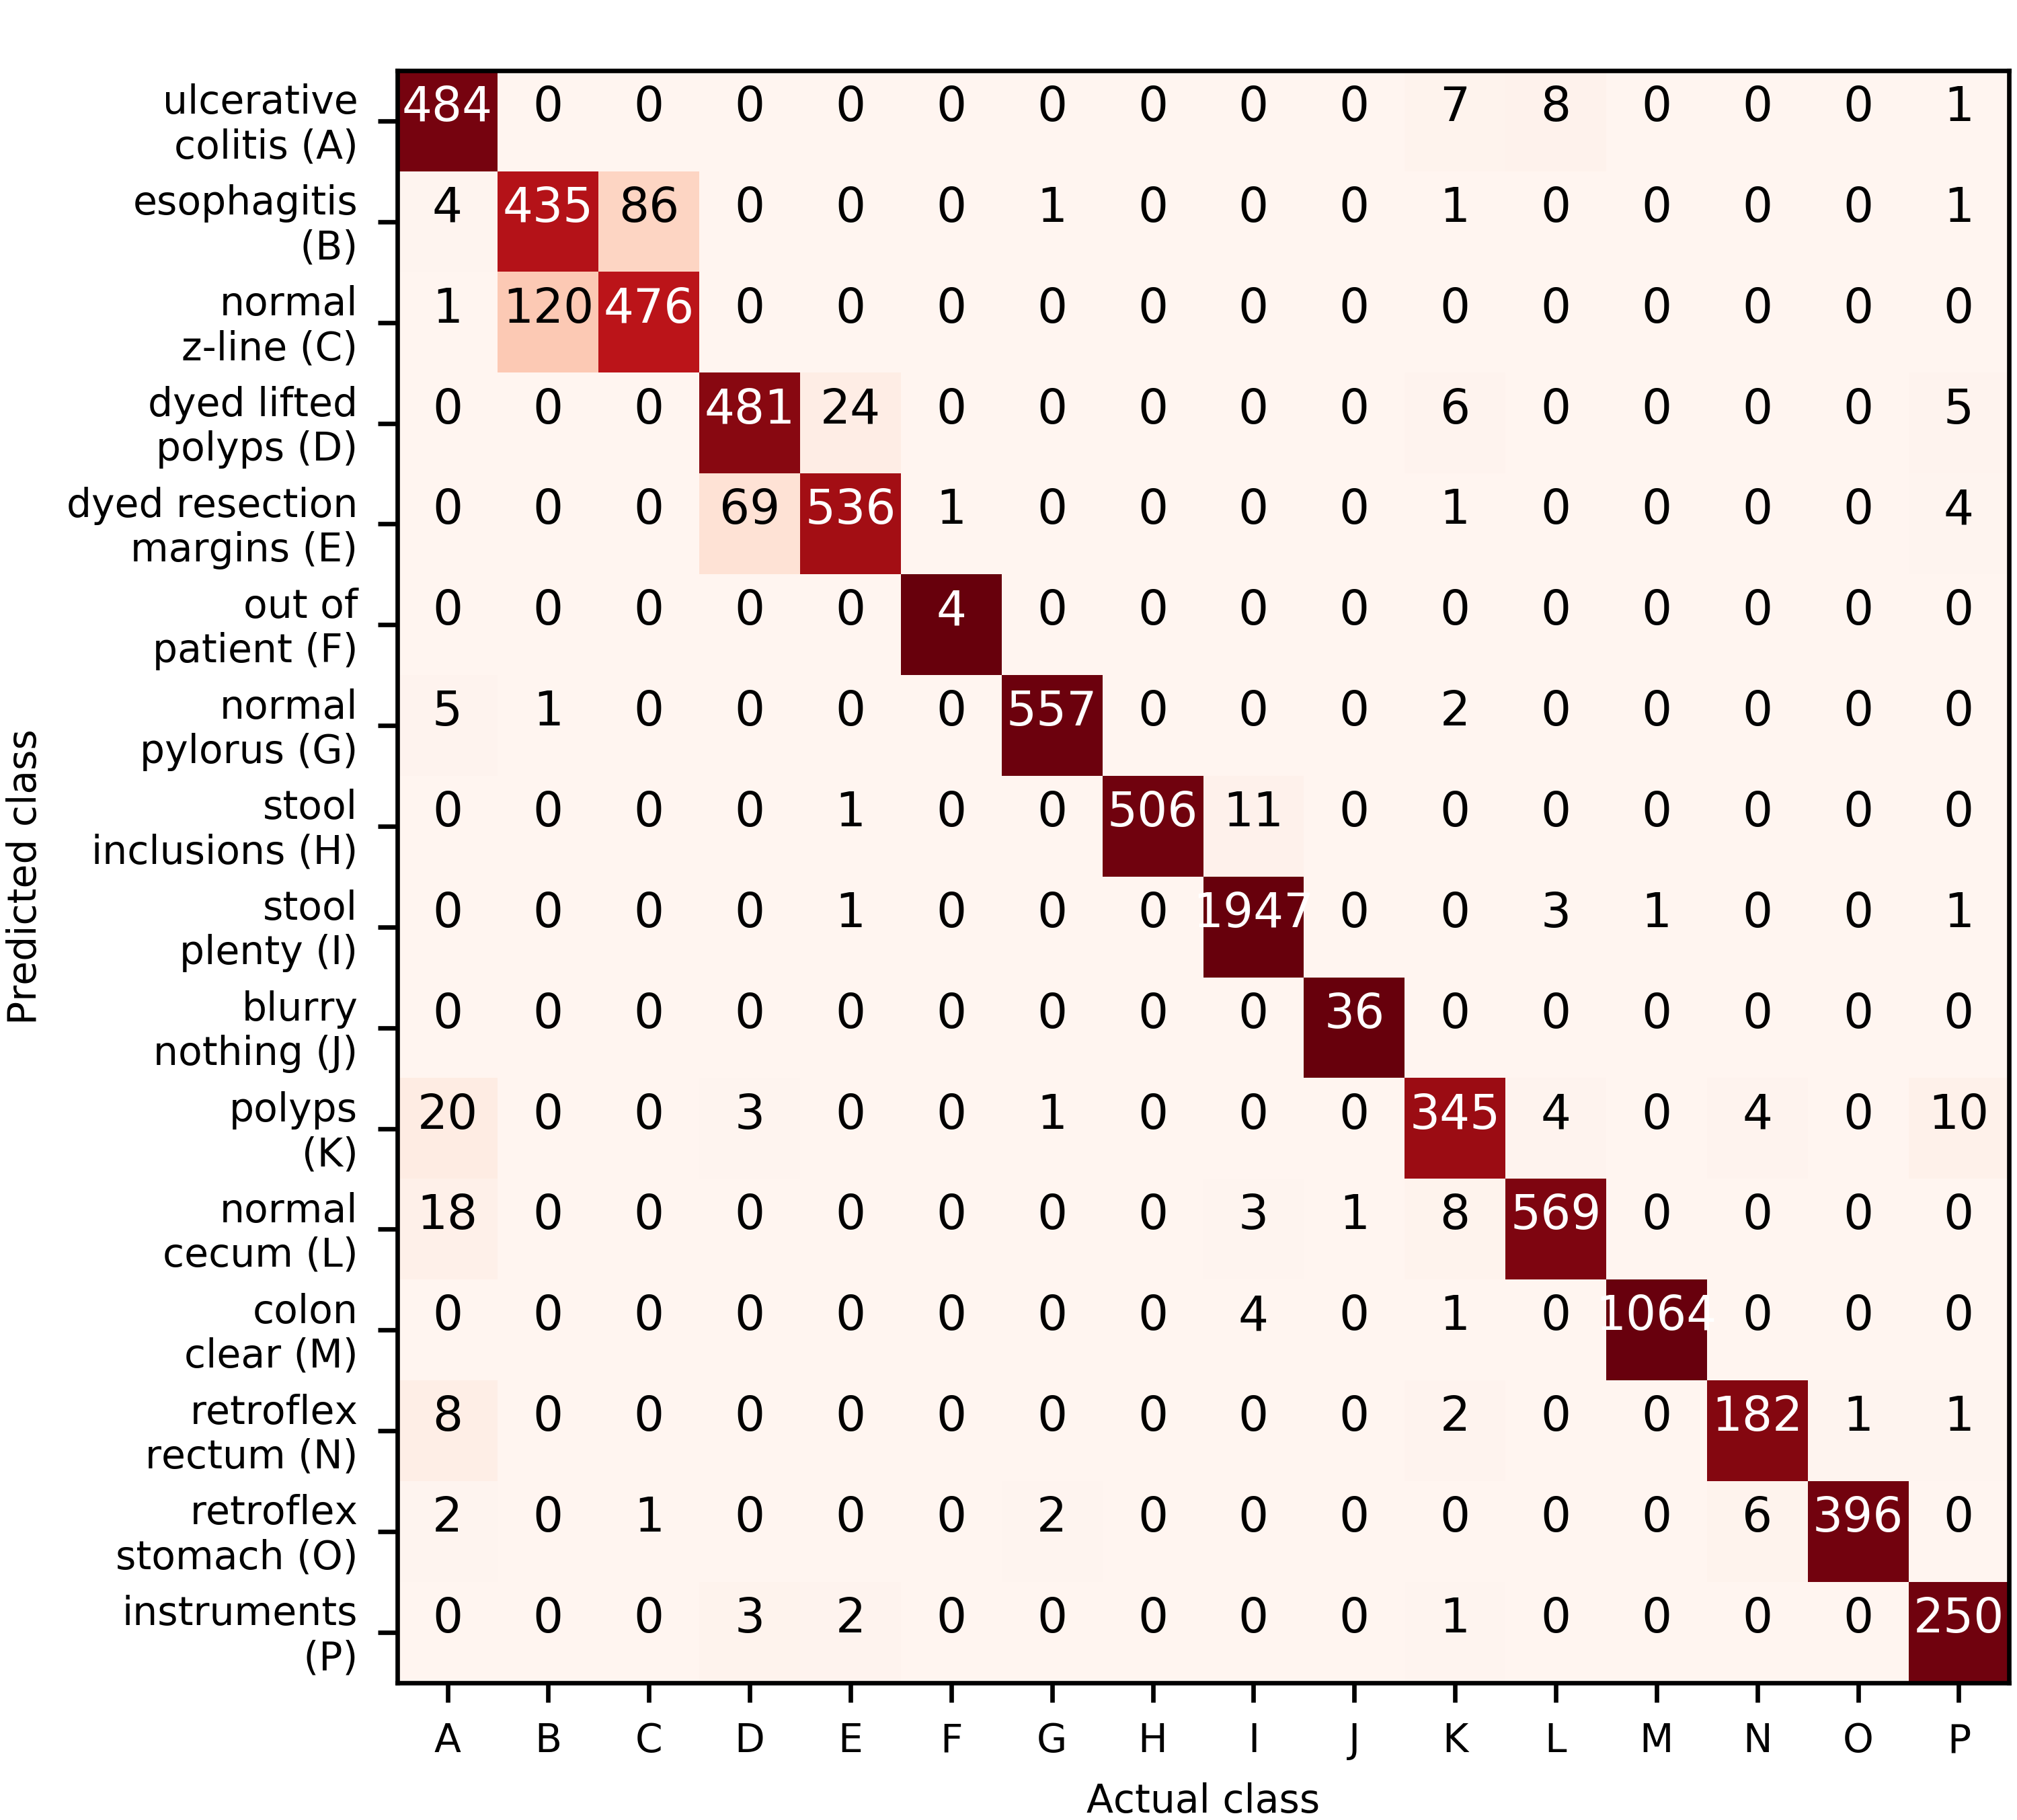
\includegraphics[width=0.8\textwidth]{endoscopy_resources/mediaeval_cfm_run3.png}
\end{center}
   \caption{The confusion matrix of our best run - \textit{Run03}.}
\label{fig:cfs_mat}
\end{figure}

\begin{table}[H]
    \caption{The official evaluation result of HCMUS team for both sub-tasks (provided by the organizers) and speed (fps) on Tesla K80 GPU}
    \centering
    \small
    \resizebox{1.0\linewidth}{!}{
    \begin{tabular}{|c|c|c|c|c|c|c|c|}
        \hline
        RunID&PREC&REC&ACC&F1&MCC&RK&FPS\\
        \hline
        Run01&94.245&94.245&99.281&94.245&93.861&93.590&6.589\\
        Run02&93.959&93.959&99.245&93.959&93.556&93.273&\textbf{23.191}\\
         \textbf{Run03}& \textbf{94.600}& \textbf{94.600}& \textbf{99.325}& \textbf{94.600}& \textbf{94.240}& \textbf{93.987}& 23.148\\
        Run04&93.043&93.043&99.130&93.043&92.579&92.257&22.654\\ 
        Run05&94.508&94.508&99.314&94.508&94.142&93.884&21.413\\
        \hline
    \end{tabular}
    \label{hcmus_result}
    }
\end{table}

\begin{table}[]
\caption{Medico: The 2018 Multimedia for Medicine Task challenge result}
\resizebox{\textwidth}{!}{
\begin{tabular}{|l|l|l|l|l|}
\hline
Rank       & Authors                                                                                   & ACC             & MCC             & Affiliation                                                                                                                                       \\ \hline
\textbf{1} & \textbf{Hoang et al.}                                                                     & \textbf{0.9933} & \textbf{0.9424} & \textbf{\begin{tabular}[c]{@{}l@{}}University of Science, VNU-HCM\\ Eurecom, France\\ University of Information Technology,\\ VNU-HCM\end{tabular}} \\ \hline
2          & Thambawita et. al.                                                                        & 0.9421          & 0.9932          & \begin{tabular}[c]{@{}l@{}}Simula Research Laboratory, Norway\\ Oslo Metropolitan University\\ University of Oslo\end{tabular}                    \\ \hline
3          & S. Hicks et. al. & 0.9350          & 0.9920          & \begin{tabular}[c]{@{}l@{}}Simula Research Laboratory\\ University of Oslo\\ Simula Metropolitan Center for \\ Digital Engineering\end{tabular}   \\ \hline
4          & R. J. Borgli et al.                                                                       & 0.9310          & -               & Simula Research Laboratory, Norway                                                                                                                \\ \hline
5          & T. H. Ko et. al. & -               & 0.9471          & \begin{tabular}[c]{@{}l@{}}University of Hong Kong, HKSAR, China\\ Hong Kong Baptist University, HKSAR, China\end{tabular}                        \\ \hline
6          & Kirkerød et al.                                                                           & 0.9110          & 0.9890          & \begin{tabular}[c]{@{}l@{}}Oslo Metropolitan University\\ University of Oslo\end{tabular}                                                         \\ \hline
7          & D. Dias et al.                                                                            & -               & 0.9880          & University of Campinas, Brazil                                                                                                                    \\ \hline
8          & M. Taschwer et al.                                                                        & 0.8942          & 0.9876          & \begin{tabular}[c]{@{}l@{}}Klagenfurt University (AAU), Austria\\ Florida Atlantic University (FAU), USA\end{tabular}                             \\ \hline
9          & Z. Khan, A. Tahir                                                                         & 0.7560          & 0.9790          & \begin{tabular}[c]{@{}l@{}}National University of Computer and \\ Emerging Sciences, Karachi Campus, Pakistan\end{tabular}                        \\ \hline
10         & M. Steiner et. al. & 0.5473          & 0.9469          & \begin{tabular}[c]{@{}l@{}}Alpen-Adria-Universität Klagenfurt, Austria\\ SimulaMet, Norway\\ University of Oslo, Norway\end{tabular}              \\ \hline
\end{tabular}}
\label{teams_result}
\end{table}


\begin{ChapAbstract}
In this chapter, we describe the results of our proposed approaches. Through experiments on endoscopic image dataset, we have shown that  simple samples augmentation mechanism can bring impressive result. Besides, utilizing the advantages of several deep learning models we can increase the overall performance of our system instead of using each of them separately. 
\end{ChapAbstract}